% ============================
% Configuración del documento
% ============================
\documentclass[stu,12pt,bbm,biblatex]{apa7}
\addbibresource{referencias.bib}

\usepackage[spanish,es-nodecimaldot]{babel}
\usepackage{csquotes}
\usepackage{graphicx}
\usepackage{enumitem}
\usepackage{fancyhdr}
\usepackage{indentfirst}
% Fuente Times New Roman 12pt
\usepackage[T1]{fontenc}
\usepackage{newtxtext,newtxmath}

% Justificación de texto y Sangría APA 7 (1.27 cm)
\usepackage{ragged2e} 
\setlength{\parindent}{1.27cm}
\makeatletter
\AtBeginDocument{
    \justifying
    \setlength{\parindent}{1.27cm}
    \renewcommand{\raggedright}{\justifying}
    \renewcommand{\RaggedRight}{\justifying}
}
\makeatother

% ==============================================
% Configuración y corrección de títulos (Niveles 2, 3 y 4)
% ==============================================
\makeatletter
% Nivel 2: Subsection (2.5. Marco Teórico y conceptual)
\renewcommand{\subsection}{%
  \@startsection{subsection}{2}{\z@}%
  {-2.5ex plus -1ex minus -.2ex}%
  {1ex plus .2ex}%
  {\normalfont\normalsize\bfseries}%
}

% Nivel 3: Subsubsection (2.5.1. Fundamento teórico...)
\renewcommand{\subsubsection}{%
  \@startsection{subsubsection}{3}{\z@}%
  {-1.8ex plus -0.5ex minus -.2ex}%
  {0.8ex plus .2ex}%
  {\normalfont\normalsize\bfseries\itshape}%
}

% Nivel 4: Subsubsubsection / Paragraph (2.5.1.1. Sistema web:)
\renewcommand{\paragraph}{%
  \@startsection{paragraph}{4}{\parindent}% Sangría de 1.27 cm alineada al párrafo
  {-1.5ex plus -0.5ex minus -.2ex}% Espacio superior
  {0.8ex plus .2ex}% Espacio inferior (positivo para dar salto de línea)
  {\normalfont\normalsize\bfseries\itshape}% Negrita y cursiva
}

% Formato numérico para el nivel 4 (ej. 2.5.1.1)
\renewcommand{\theparagraph}{\thesubsubsection.\arabic{paragraph}}

% Alias para que puedas usar directamente \subsubsubsection en tu documento
\newcommand{\subsubsubsection}{\paragraph}
\makeatother

% IMPORTANTE: Cambiar de 3 a 4 para que LaTeX numere el nivel 2.5.1.1
\setcounter{secnumdepth}{4}
\setcounter{tocdepth}{4}

% ============================
% Numeración y encabezados
% ============================
\pagestyle{fancy}
\fancyhf{}
\fancyfoot[C]{\thepage}
\renewcommand{\headrulewidth}{0pt}
\renewcommand{\footrulewidth}{0pt}

\fancypagestyle{plain}{
    \fancyhf{}
    \fancyfoot[C]{\thepage}
    \renewcommand{\headrulewidth}{0pt}
    \renewcommand{\footrulewidth}{0pt}
}

% ====================
% Portada de capítulos
% ====================
\newcommand{\portadacapitulo}[1]{
    \clearpage
    \refstepcounter{section}
    \thispagestyle{plain}
    \vspace*{\fill}
    \begin{center}
        {\Large\bfseries CAPÍTULO \arabic{section}}\\[0.4cm]
        {\LARGE\bfseries #1}
    \end{center}
    \vspace*{\fill}
    \addcontentsline{toc}{section}{CAPÍTULO \arabic{section}: #1}
    \clearpage
}

\shorttitle{Sistema web de planillas}

\begin{document}

    % ============================
    % PORTADA INSTITUCIONAL SENATI
    % ============================
    \begin{titlepage}
        \thispagestyle{empty}
        \centering
        
        % Logo ampliado
        
\includegraphics[width=0.72\linewidth]{images/senati_logo.png} 
        
        \vspace{0.3cm}
        {\bfseries\large SERVICIO NACIONAL DE ADIESTRAMIENTO EN TRABAJO INDUSTRIAL} \\[0.25cm]
        {\bfseries DIRECCIÓN ZONAL: LIMA – CALLAO} \\[0.2cm]
        {\small ESCUELA DE TECNOLOGÍA DE LA INFORMACIÓN} \\[0.15cm]
        {\small CFP LUIS CÁCERES GRAZIANI} \\[0.15cm]
        {\small DESARROLLO DE SOFTWARE} 

        \vfill

        {\normalsize Proyecto de Innovación y/o Mejora} \\[0.15cm]
        {\normalsize Nivel Profesional Técnico / Técnico Operativo} 

        \vfill

        {\bfseries\large ``Desarrollo e implementación de un sistema web con flujos automatizados\\
            para la gestión de nóminas y procesos de recursos humanos\\
            orientado a clientes empresariales de J~\&~P~Periféricos~S.A.C.''\par}

        \vfill

        {\bfseries Autores:} \\[0.15cm]
        {\normalsize Daniel Enrique Singer Rojas} \\[0.1cm]
        {\normalsize Rodrigo Alessandro Castillo Del Castillo} \\[0.1cm]
        {\normalsize Adrian Matias Dueñas Huertas} 

        \vfill

        {\bfseries Asesor:} \\[0.15cm]
        {\normalsize Mg. Jose Armando Tiznado Ubillus} 

        \vfill

        \textbf{Lima – Perú} \\[0.15cm]
        \textbf{2026}
    \end{titlepage}
    \setcounter{page}{2}

    % ============================
    % DEDICATORIA Y AGRADECIMIENTOS
    % ============================
    \clearpage
    \phantomsection
    \addcontentsline{toc}{section}{Agradecimiento}
    \noindent{\bfseries\large Agradecimiento} \\[0.5cm]
    Agradezco sinceramente a nuestro asesor, el Mg. José Tiznado, y al docente Omar Espinoza por su orientación metodológica y retroalimentación técnica. A mis compañeros de tesis por el esfuerzo y compromiso compartido en esta meta profesional; a Melanie y Gianella por su valioso apoyo en los procesos de RR.HH. y diseño UI/UX del sistema; a Dylan por su ayuda con la documentacion inicial y arquitectura del proyecto; y a J\,\&\,P Periféricos S.A.C. por la confianza y el espacio brindado para desarrollar este proyecto en un entorno real.

\begin{flushright}
    \small\textit{--- Daniel Enrique Singer Rojas}
\end{flushright}
    Agradezco a todos los instructores que tuve a lo largo de mi carrera en SENATI por compartir sus conocimientos. De manera especial, agradezco a nuestro asesor, el Mg. José Tiznado, por guiarnos y apoyarnos en nuestra tesis, y al instructor Omar Espinoza por enseñarnos más de lo exigido en SENATI. También agradezco a mis compañeros de tesis por recibirme en su equipo y por el gran esfuerzo que le dedicaron en este proyecto. 

\begin{flushright}
    \small\textit{--- Rodrigo Alessandro Castillo Del Castillo}
\end{flushright}
    Presento mi agradecimiento al asesor, Omar Espinoza, por su buena orientación en el ámbito técnico; a Dylan, por su ayuda en la toma de decisiones en el proyecto; y a J\&P Periféricos S.A.C., por la confianza para desarrollar las habilidades técnicas en el entrorno laboral real.

\begin{flushright}
    \small\textit{--- Adrian Matias Dueñas Huertas}
\end{flushright}

    
    \clearpage
    \phantomsection
    \addcontentsline{toc}{section}{Dedicatoria}
    \noindent{\bfseries\large Dedicatoria} \\[0.5cm]
    Dedico este proyecto a todas las personas que han formado parte de mi camino y me han brindado su constante apoyo y motivación para alcanzar esta meta: a mi familia, compañeros y amigos más cercanos. Y De manera especial, a la comunidad de \textit{Twenty One Pilots Perú}, por impulsarme a salir de mi zona de confort y a confiar plenamente en mí mismo. \textit{Stay Alive}

\begin{flushright}
    \small\textit{--- Daniel Enrique Singer Rojas}
\end{flushright}
    Dedico este proyecto a mi familia la cual me ha estado apoyando en toda mi trayectoria en SENATI, además a mis compañeros los cuales me han ayudado ya sea de manera directa o indirecta a levantarme el ánimo cuando más lo necesitaba.

\begin{flushright}
    \small\textit{--- Rodrigo Alessandro Castillo Del Castillo}
\end{flushright}
    Dedico este proyecto a mi madre, padre, hermana y compañeros que me han apoyado en el transcurso de estudiante en SENATI, dándome consejos e  impulsarme a la mejora continua de mi persona.
\begin{flushright}
    \small\textit{--- Adrian Matias Dueañas Huertas}
\end{flushright}

    % ============================
    % ÍNDICES
    % ============================
    \clearpage
    \tableofcontents

    \clearpage
    \listoffigures

    \clearpage


    % ============================
    % PRELIMINARES
    % ============================
    \input{portada/resumen}
    \clearpage
\phantomsection
\addcontentsline{toc}{section}{Introducción}

{\centering\Large\bfseries INTRODUCCIÓN\par}
\vspace{0.8cm}

En el entorno empresarial contemporáneo, la administración de los empleados y el procesamiento de compensaciones constituyen procesos críticos para la continuidad operativa. No obstante, una gran parte de las organizaciones continúa gestionando sus planillas mediante hojas de cálculo convencionales. Este enfoque tradicional demanda una inversión desmedida de tiempo en la validación manual de asistencias, permisos, bonificaciones y deducciones de ley, lo que incrementa sustancialmente el margen de error humano en el cálculo de la planilla, generando retrasos en la dispersión de fondos, pagos inexactos y potenciales contingencias laborales. Asimismo, el almacenamiento de información financiera en archivos planos o locales expone a las organizaciones a graves riesgos de fuga de datos o accesos no autorizados.

Frente a este escenario, el presente proyecto de innovación propone el diseño e implementación de un sistema web integral bajo una arquitectura de despliegue monolítica modular, orientado a centralizar la gestión de personal y automatizar el cálculo sistemático de planillas. Para optimizar el ciclo operativo, la plataforma se integra con la herramienta de orquestación y automatización de flujos \textbf{n8n}, la cual procesa la dispersión de pagos y gestiona el envío automatizado de las boletas de pago digitales a las casillas de correo electrónico de cada colaborador.

Con el fin de garantizar la confidencialidad, integridad y disponibilidad de los datos sensibles, el sistema incorpora un modelo riguroso de control de acceso basado en roles (RBAC), mecanismos de cifrado \textbf{AES-256-GCM} para los registros financieros sensibles y un módulo de auditoría continua que registra la trazabilidad completa de cada transacción y cambio de estado ejecutado en la plataforma.

    % ============================
    % CAPÍTULOS
    % ============================
    % ===============================
% Pagina principal del capitulo 1
% ===============================
\portadacapitulo{GENERALIDADES DE LA EMPRESA}

\subsection{Datos Generales de la Empresa}

\subsubsection{Reseña histórica de la empresa}
J\&P Periféricos S.A.C. es una empresa peruana del sector informático que inició sus operaciones el 1 de octubre del año 2011. Su propósito es brindar soluciones informáticas a empresas cuyas necesidades son la mejora de sus procesos internos. Asimismo, ofrece la venta de productos tecnológicos tanto a personas naturales como empresas.

Con el paso de los años, J\&P Periféricos fue logrando consolidar su presencia en el sector y especializando sus soluciones de acuerdo a las necesidades de sus clientes. Además, ha ampliado el alcance de sus servicios, dando mantenimiento y soporte técnico continuo con el fin de alcanzar una mayor credibilidad y mejorar la relación con sus clientes.

\subsubsection{Quiénes Somos}
J\&P Periféricos S.A.C. es una empresa peruana en el rubro de la informática que brinda soluciones integrales informáticas tales como el mantenimiento informático, venta de productos tecnológicos, desarrollo de páginas web, redes y comunicaciones, empleando tecnología actual para una mejor eficiencia y rapidez en sus procesos.

\subsubsection{Razón Social}

{
    \centering
    \renewcommand{\arraystretch}{1.35}
    \setlength{\tabcolsep}{4pt}
    \begin{tabular}{
        @{}
        p{2.8cm}
        p{4.8cm}
        @{\hspace{0.2cm}}
        p{2.8cm}
        p{4.8cm}
        @{}
    }
        \textbf{Empresa} & 
        J\&P Periféricos S.A.C. & 
        \textbf{Empresario} 
        & Julio Flores Vicuña 
        \\[2pt]
        
        \textbf{RUC} &
        20545122520 &
        \textbf{Rubro} &
        Soluciones Informáticas
        \\[5pt]
        
        \textbf{Distrito} &
        Cercado de Lima & 
        \textbf{Dirección} &
        {\raggedright Jr. Emilio Fernández 160 Dpto. 1804\par}
        \\
    \end{tabular}
    \par
}
\clearpage
\subsubsection{Logo de la Empresa}

\begin{center}
    \vspace{0.1cm}
    %  Identificador y título en formato APA 7
    \refstepcounter{figure}
    \label{fig:logo_empresa}

    \addcontentsline{lof}{figure}{%
        Figura~\thefigure. Logotipo institucional de
        J\&P Periféricos S.A.C.}

    {\bfseries Figura~\thefigure}\par\vspace{0.1cm}
    {\itshape Logotipo institucional de J\&P Periféricos S.A.C.}\par
    \vspace{0.25cm}

    % Imagen del logo
    
\includegraphics[width=0.52\linewidth]{images/J&P_Logo.png}\par
    \vspace{0.25cm}

    % Nota explicativa alineada al ancho de la imagen
    \begin{minipage}{0.52\linewidth}
        \small
        \textit{Nota.} Gráfico representativo del logotipo corporativo de la empresa.
    \end{minipage}
\end{center}

\subsubsection{Ubicación de la Empresa}

La sede de \textbf{J\&P Periféricos S.A.C.} se encuentra ubicada en el departamento Concepto Urbano Plus, Calle Emilio Fernández 160, Dpto. 1804, distrito de Cercado de Lima (Código Postal 15046). Como referencia de acceso principal, el inmueble se ubica a la altura de la cuadra 8 de la Avenida Arequipa.

\begin{center}
    % Título formato APA 7 (Recto / Sin cursiva)
    \refstepcounter{figure}
    \label{fig:ubicacion_empresa}
    \addcontentsline{lof}{figure}{%
        Figura~\thefigure.
        Localización y vías de acceso de la empresa}

    {\bfseries Figura~\thefigure}\par
    {\itshape Localización y vías de acceso de la empresa}\par
    \vspace{0.20cm}

    % Imagen con borde gris tenue
    {\color{gray!60}\setlength{\fboxsep}{0pt}\setlength{\fboxrule}{0.6pt}%
    \fbox{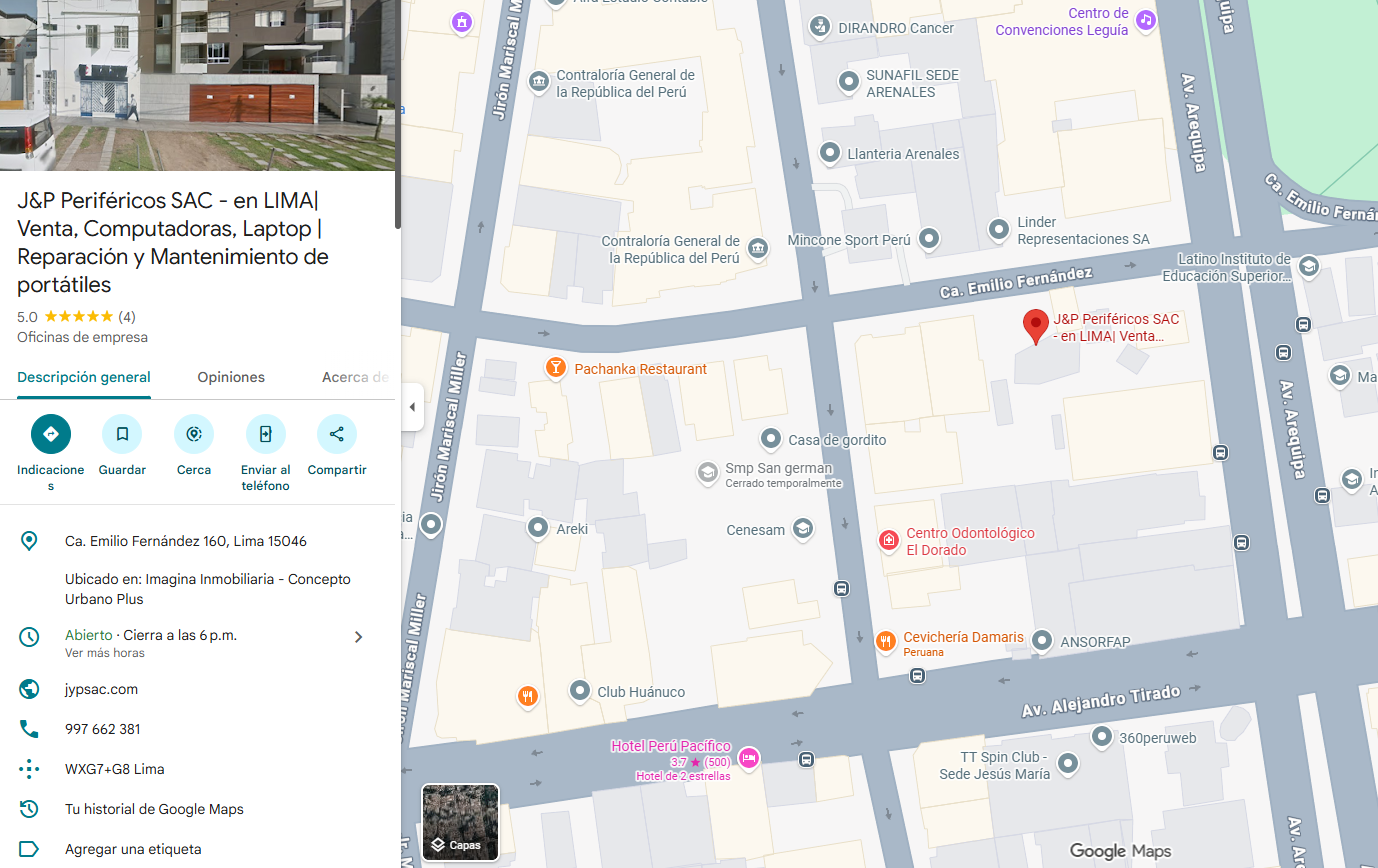
\includegraphics[width=0.90\linewidth, height=6cm, keepaspectratio=false]{images/ubicacion_empresa.png}}}\par
    \vspace{0.25cm}

    % Nota APA 7 alineada al ancho de 0.90
    \begin{minipage}{0.90\linewidth}
        \small
        \textit{Nota.} Ubicación geográfica y mapa vial de la sede central. Adaptado de Google Maps.
    \end{minipage}
\end{center}

% ===============================================================
% Seccion 1.2: Mision, Vision, Objetivos y valores de la empresa
% ===============================================================
\subsection{Misión, Visión, Objetivos, Valores de la Empresa}

% ==========================Mision=====================================
\subsubsection{Misión}
Proporcionar soluciones tecnológicas orientadas a la optimización de los procesos de negocio, facilitando a los clientes métodos efectivos para afrontar los desafíos informáticos empresariales mediante la implementación estratégica y adecuada de las tecnologías de la información.

% ==========================Vision=====================================

\subsubsection{Visión}
Posicionarse como una organización referente en soluciones informáticas, altamente eficiente y rentable, operando bajo estándares de calidad internacional, con un equipo humano calificado y un firme compromiso con el desarrollo sostenible y la preservación del medio ambiente, garantizando la expansión y continuidad del negocio.

% ==========================Objetivos=====================================

\subsubsection{Objetivos de la Empresa}

% Objetivos a corto plazo
\noindent\textbf{Objetivos a Corto Plazo:}
\begin{itemize}
    \item Consolidar la presencia y posicionamiento comercial en el mercado peruano.
    \item Ampliar la cartera de clientes corporativos e individuales.
    \item Diversificar y actualizar el portafolio de servicios tecnológicos.
    \item Incrementar los índices de satisfacción y fidelización de los clientes.
    \item Optimizar los flujos operativos y tiempos de respuesta en los procesos internos.
\end{itemize}

% Objetivos a largo plazo

\noindent\textbf{Objetivos a Largo Plazo:}
\begin{itemize}
    \item Posicionarse como una empresa líder e innovadora en el sector de tecnologías de la información.
    \item Asegurar la sostenibilidad financiera y la escalabilidad operativa del modelo de negocio.
    \item Contribuir activamente a la transformación digital y al desarrollo tecnológico nacional.
\end{itemize}

% Valores de la empresa

\subsubsection{Valores de la Empresa}

\begin{itemize}
    \item \textbf{Orientación al cliente:} Atención focalizada en los requerimientos específicos de cada cliente, diseñando soluciones a medida que potencien sus procesos de negocio.
    \item \textbf{Innovación continua:} Adopción y aplicación proactiva de tecnologías emergentes para generar valor agregado y dinamismo operativo.
    \item \textbf{Calidad y excelencia:} Compromiso con la entrega de productos y servicios que cumplan con altos estándares técnicos y de rendimiento.
    \item \textbf{Desarrollo humano:} Fomento del crecimiento profesional, técnico y personal del capital humano como pilar del éxito organizacional.
    \item \textbf{Responsabilidad social y ambiental:} Conciencia ambiental y ética corporativa orientada al desarrollo sostenible y buenas prácticas operativas.
\end{itemize}
\subsection{Producto, Mercado y Cliente}

\subsubsection{Producto}
La empresa \textbf{J\&P Periféricos S.A.C.} comercializa una gama integral de equipamiento informático, 
suministros y soluciones tecnológicas orientadas tanto al usuario final como al sector corporativo de Lima Metropolitana. Su portafolio de productos y servicios incluye:

\begin{itemize}
    \item \textbf{Laptops y Tablets:} Equipos portátiles para uso personal, profesional y entornos de alto rendimiento.
    \item \textbf{PC y Servidores:} Computadoras de escritorio ensambladas a medida y estaciones de trabajo o servidores para infraestructura empresarial.
    \item \textbf{Impresoras:} Equipos de impresión multifuncionales, térmicos y de inyección o láser para oficina.
    \item \textbf{Monitores:} Pantallas y soluciones de visualización con diversas resoluciones y tecnologías de panel.
    \item \textbf{Componentes para PC:} Placas base, procesadores, memorias RAM, tarjetas de video y unidades de almacenamiento en estado sólido (SSD).
    \item \textbf{Accesorios y Repuestos:} Periféricos de entrada/salida, cables estructurados, fuentes de poder y partes de recambio.
    \item \textbf{Soluciones Corporativas:} Servicios de integración tecnológica, mantenimiento preventivo/correctivo y soporte continuo de infraestructura TI.
\end{itemize}

Como parte de la diversificación de su portafolio tecnológico, J\&P Periféricos S.A.C. ha encargado el desarrollo de un sistema web para la gestión de nóminas y procesos administrativos de recursos humanos. La empresa proyecta ofrecer esta solución a clientes empresariales mediante una modalidad de suscripción. El presente proyecto comprende el desarrollo y la validación de la solución; su comercialización se plantea como una etapa
posterior.

\subsubsection{Mercado}
El mercado objetivo de la organización se enmarca dentro del sector de las Tecnologías de la Información y Comunicación (TIC). La oferta está dirigida principalmente al segmento empresarial (B2B) y a profesionales independientes (B2C) en Lima Metropolitana que requieren aprovisionamiento de hardware, despliegue de redes, mantenimiento de infraestructura informática y optimización técnica de sus procesos de negocio mediante herramientas digitales.

Para el producto desarrollado en este proyecto, los destinatarios previstos son empresas que requieren integrar la información laboral de sus trabajadores con el procesamiento de nóminas, la revisión de incidencias y la generación de documentos. La cartera existente constituye un ámbito potencial para identificar usuarios interesados, sin que ello implique que todos sus integrantes hayan solicitado o contratado la solución.

\subsubsection{Cliente}
La cartera de clientes de \textbf{J\&P Periféricos S.A.C.} abarca diversas entidades comerciales, industriales, de salud y servicios profesionales, entre las cuales destacan:

\begin{itemize}
    \item Grupo Enfoque
    \item Sergetic
    \item S\&R Solution Service
    \item Hidromax S.A.C.
    \item Copaco S.A.C.
    \item Fasetron del Perú S.A.C.
    \item Asociación Peruana de Nefrología Pediátrica
    \item Distribuidora Venso S.A.C.
    \item Textiles TBM S.A.C.
\end{itemize}
\clearpage
\subsection{Organigrama de la Empresa}

\begin{center}
    \vspace{0.3cm}
    % Título formato APA 7
    \refstepcounter{figure}
    \label{fig:organigrama}
    \addcontentsline{lof}{figure}{%
        Figura~\thefigure.
        Estructura orgánica funcional de J\&P Periféricos S.A.C.}

    {\bfseries Figura~\thefigure}\par\vspace{0.1cm}
    {\itshape Estructura orgánica funcional de J\&P Periféricos S.A.C.}\par
    \vspace{0.20cm}

    % Organigrama con borde (ancho 0.98 para evitar advertencia de desborde de margen)
    {\color{gray!60}\setlength{\fboxsep}{0pt}\setlength{\fboxrule}{0.6pt}%
    \fbox{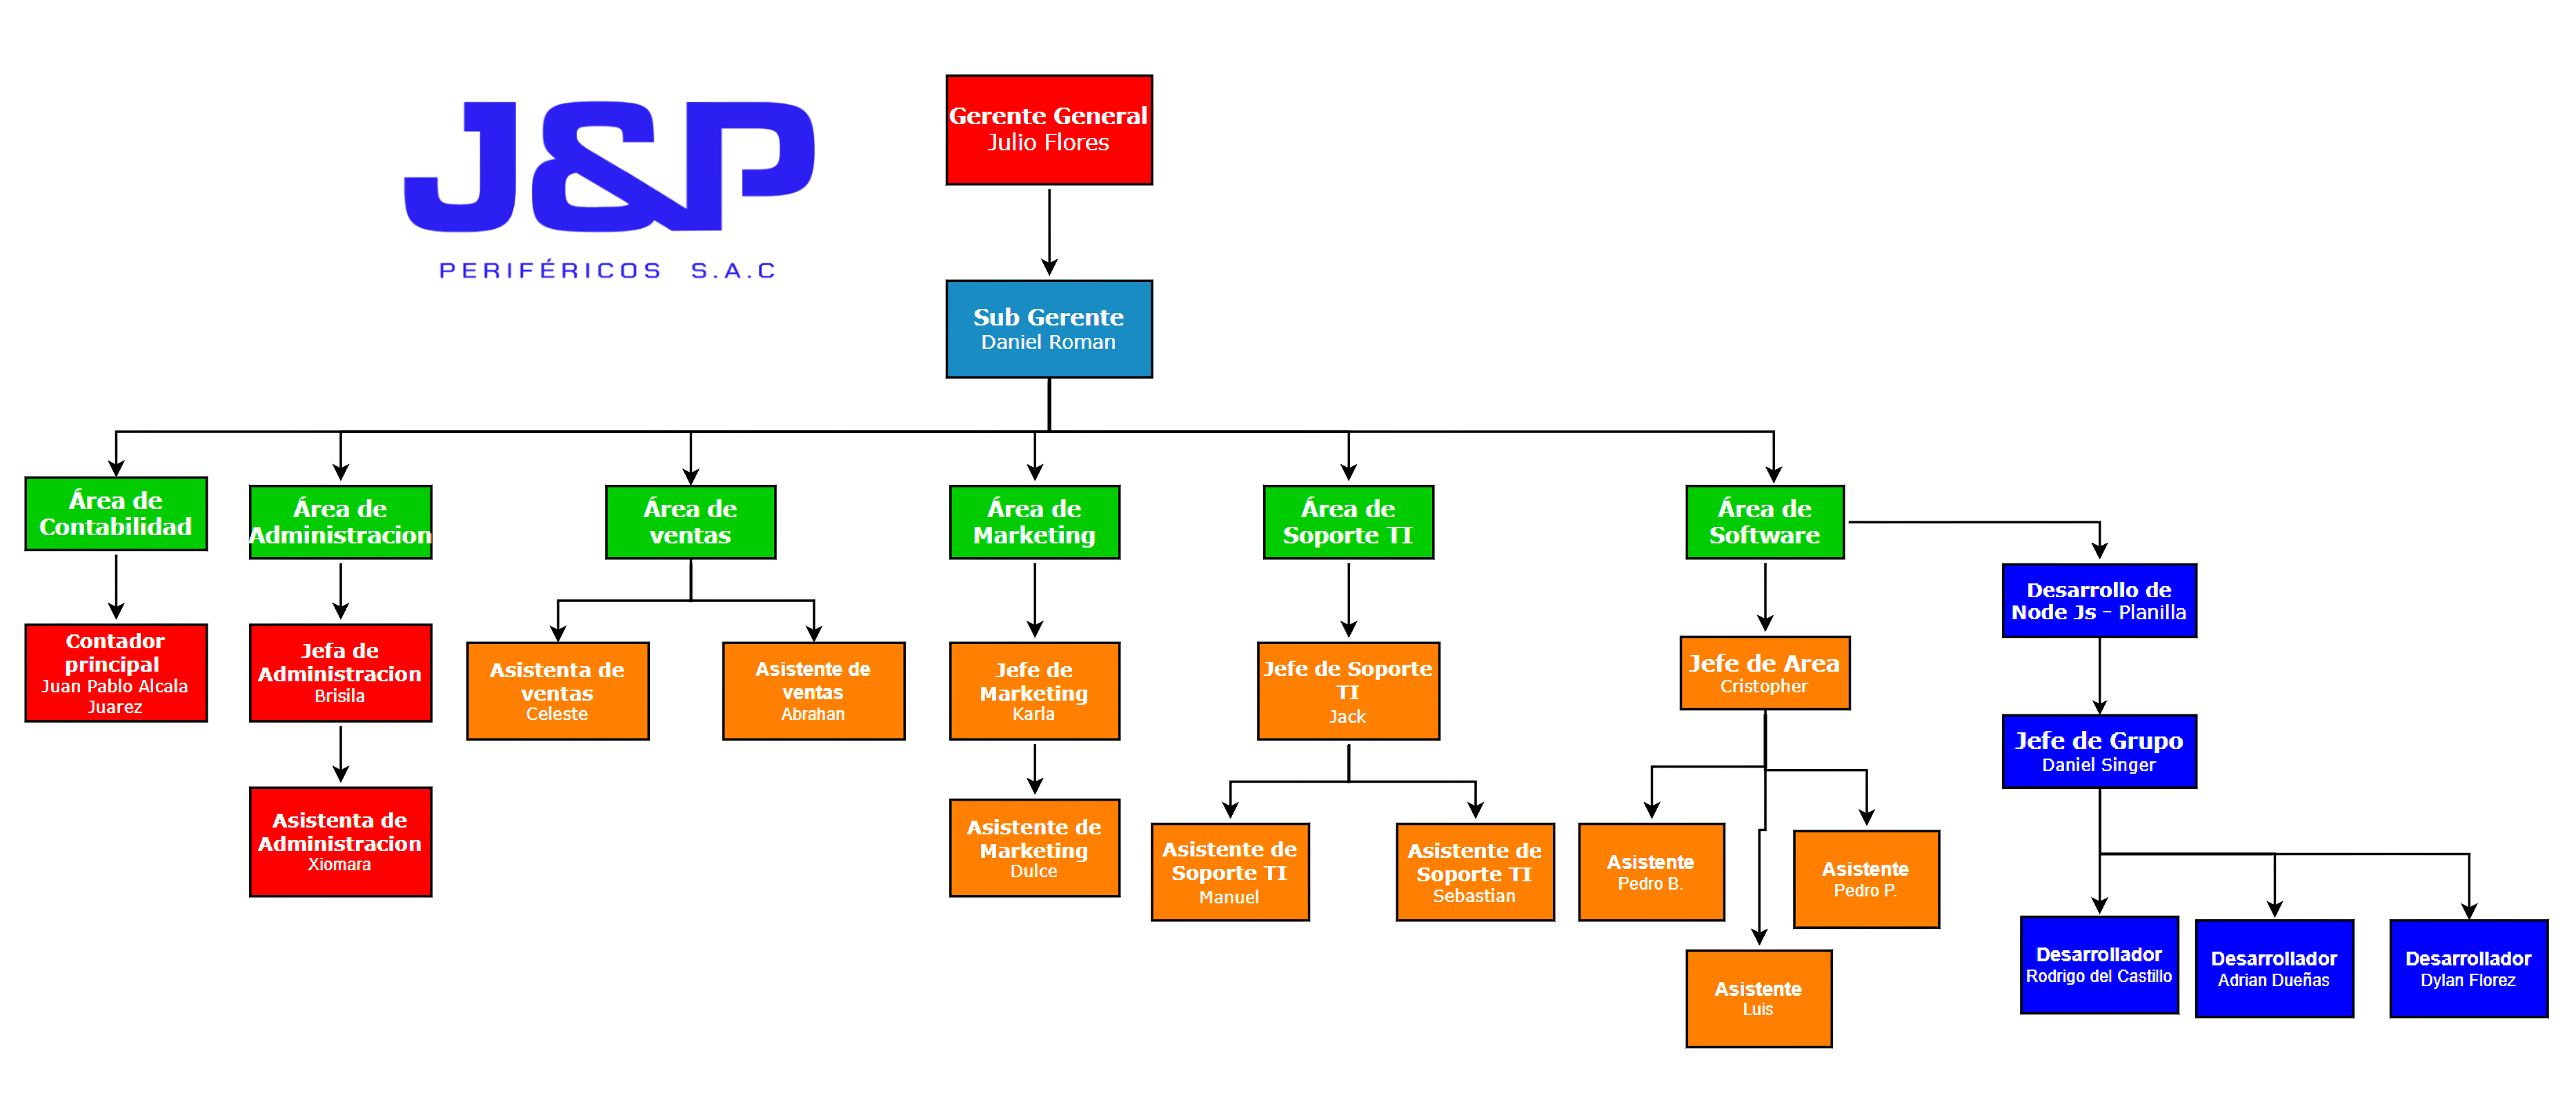
\includegraphics[width=1\linewidth]{images/organigrama.png}}}\par
    \vspace{0.25cm}

    % Nota APA 7 alineada al ancho de 0.98
    \begin{minipage}{0.98\linewidth}
        \small
        \textit{Nota.} Representación jerárquica y departamental de las áreas funcionales de la empresa. Elaboración propia.
    \end{minipage}
\end{center}

\subsection{Otra información relevante de la empresa donde se desarrolla el proyecto}

\subsubsection{Planificación y gestión de la entrevista}

Con el propósito de profundizar en el diagnóstico situacional, contrastar la perspectiva estratégica del negocio y sustentar las causas raíz de las deficiencias operativas en el cálculo de haberes, se diseñó e implementó una entrevista semiestructurada aplicada a los responsables directos de la gestión empresarial y financiera.

\vspace{0.3cm}
\noindent\textbf{Entrevistado:} Julio Flores Vicuña, \textbf{Gerente General de J\&P Periféricos S.A.C.}
\vspace{0.4cm}

\begin{enumerate}[leftmargin=*, label=\textbf{P\arabic*.}]
    \item \textbf{¿Cuáles son las principales dificultades de gestión interna que ha identificado en las empresas de su cartera de clientes?}
    
    \textit{Respuesta del Gerente General:} Los principales inconvenientes son los errores en cálculos de nómina, retrasos en pagos, registros imprecisos de horas/licencias y falta de integración tecnológica. Estos problemas generan reclamos, sanciones de SUNAFIL y pérdida de confianza en los equipos.

    \item \textbf{¿Qué motivos estratégicos llevaron a la empresa a optar por el desarrollo de una solución propia de planillas en lugar de contratar un software comercial existente?}
    
    \textit{Respuesta del Gerente General:} Un sistema de planillas personalizado permite a una empresa con muchos empleados reducir errores, cumplir con normativas locales (SUNAT/SUNAFIL), y adaptar cálculos a sus propias políticas de bonos, turnos y beneficios. Además, ofrece mayor seguridad de datos y flexibilidad frente a cambios legales o internos.

    \item \textbf{Desde su perspectiva como gerente, ¿cuáles representan los mayores desafíos al momento de supervisar el cumplimiento, asistencias e incidencias de los colaboradores?}
    
    \textit{Respuesta del Gerente General:} Tener la información actualizada en tiempo real de los integrantes de cada proceso y medir su desempeño.

    \item \textbf{¿Qué impacto operativo y económico espera que genere este sistema, tanto a nivel interno en J\&P Periféricos como para su futura comercialización?}
    
    \textit{Respuesta del Gerente General:} En el tema operativo mejoraríamos el orden de personal asignado a los procesos y en lo económico el recupero es a mediano plazo, recuperamos la inversión, con los costos que va a reducir el sistema.

    \item \textbf{¿Qué necesidades o problemáticas administrativas comunes comparten las empresas a las que estará orientada la venta del sistema?}
    
    \textit{Respuesta del Gerente General:} Manejo de personal es un problema general en las empresas que manejan proyectos de gran envergadura, cada empresa maneja su personal de acuerdo con los contratos; los contratos definen mucho la política de pago orientado en el sistema.
\end{enumerate}

\vspace{0.3cm}
\noindent\textbf{Entrevistado:} Juan Pablo Alcalá Juárez, \textbf{Contador de una de las empresas de la cartera de clientes de J\&P Periféricos S.A.C.}
\vspace{0.4cm}

\begin{enumerate}[leftmargin=*, label=\textbf{P\arabic*.}]
    \item \textbf{¿Cuánto tiempo promedio invierte mensualmente en el proceso completo de elaboración y validación de la planilla?}
    
    \textit{Respuesta del Contador:} Aproximadamente 5 horas, considerando la revisión de las incidencias de los colaboradores, el cálculo de las remuneraciones, la preparación de los archivos de pago, la generación y distribución de las boletas. 
    También considerando el tiempo de revisión de los cálculos y la verificación de la información antes de su envío a SUNAT y a los bancos.

    \item \textbf{¿Cuáles son las fases o variables (cálculo de horas extra, tardanzas, CTS, retenciones de ley) que demandan mayor tiempo y esfuerzo manual? }
    
    \textit{Respuesta del Contador:} La revisión de las incidencias y la verificación de los datos que se utilizarán para calcular la planilla. Es necesario comprobar las horas extras, tardanzas, 
    permisos e inasistencias, y verificar que correspondan al trabajador y al periodo adecuado. 
    Cuando se encuentran diferencias o información incompleta, se requiere consultar con Recursos Humanos y corregir los registros antes de continuar con los cálculos.
    
    \item \textbf{¿El proceso de elaboración de planilla lo realiza de manera individual o cuenta con el soporte de asistentes contables?}
    
    \textit{Respuesta del Contador:} Realizo el proceso con el apoyo de un asistente contable y del encargado de Recursos Humanos.

    \item \textbf{En caso de contar con apoyo, ¿cómo se distribuyen las tareas operativas (revisión de asistencia, cálculo de incidencias, digitación)? }
    
    \textit{Respuesta del Contador:} Al asistente contable le asigno la revisión de las incidencias y la digitación de los datos, 
    mientras que yo me encargo de realizar los cálculos y revisar los resultados. 
    Una vez revisada la planilla, le encargo al asistente la generación de los archivos de pago y las boletas.

    \item \textbf{¿Cuáles son los errores o inconsistencias más frecuentes al trabajar en hojas de cálculo y qué consecuencias conllevan al momento de efectuar los desembolsos? }
    
    \textit{Respuesta del Contador:} Los errores más frecuentes son el ingreso de datos incorrectos, la omisión de incidencias como tardanzas, permisos o inasistencias, y algunos casos de duplicación de registros. Estas inconsistencias pueden generar que nos demoremos en realizar los pagos, también la posibilidad de recibir sanciones por parte de SUNAFIL y pérdida de confianza por parte de los colaboradores.

\end{enumerate}


    % ===============================
% Pagina principal del capitulo 2
% ===============================
\portadacapitulo{Plan del proyecto de innovación / Mejora / Creatividad}

\subsection{Identificación del problema técnico en la empresa}

\subsubsection{Problemática local}

\textbf{J\&P Periféricos S.A.C.}, como empresa proveedora de soluciones informáticas, ha encargado el desarrollo de un sistema de planillas que proyecta incorporar a su portafolio y ofrecer mediante suscripción a clientes empresariales. En este contexto, el problema técnico abordado consiste en desarrollar y validar una solución que integre el procesamiento de nóminas con la administración de la información laboral necesaria para su elaboración.
Según la entrevista al gerente general, las necesidades consideradas incluyen el registro de horas y licencias, la actualización de la información del personal y la integración tecnológica de los procesos. Estas observaciones orientan el levantamiento de requisitos de la solución. El proyecto no presupone que todas las empresas de la cartera presenten las mismas dificultades ni atribuye a J\&P incidentes internos de pago que no hayan sido documentados.
La propuesta comprende la centralización de registros personales, contractuales y remunerativos; la validación de entradas; el cálculo de nóminas; y la revisión de resultados mediante responsabilidades diferenciadas de Recursos Humanos y Contabilidad. Asimismo, incorpora control de acceso, historial de modificaciones y flujos automatizados para preparar archivos de pago y distribuir boletas. Su aporte se evaluará mediante pruebas funcionales y casos de cálculo definidos, distinguiendo los resultados comprobados de los beneficios esperados de su futura utilización comercial.

\subsubsection{Problemática nacional}

En el ámbito peruano, diversas organizaciones enfrentan serias complicaciones en la administración de su capital humano y nóminas debido a la persistente dependencia de hojas de cálculo convencionales y métodos manuales de registro. De acuerdo con \textcite{elperuano2026}, las inconsistencias más recurrentes en la gestión de compensaciones comprenden transferencias fuera de cronograma, dispersiones salariales incompletas y un cómputo inexacto de horas laborales, permisos y beneficios de ley, todo ello derivado de un bajo nivel de automatización en los flujos administrativos. Esta falta de estandarización técnica no solo expone a las organizaciones a contingencias administrativas y sanciones laborales, sino que afecta directamente la motivación, confianza y estabilidad de los colaboradores.

\subsubsection{Problemática internacional}

A escala global, la transición de procesos manuales hacia plataformas digitales integradas constituye un factor clave para la sostenibilidad y competitividad de las organizaciones. Según reportes del \textcite{bancomundial2024}, la adopción de herramientas tecnológicas incrementa de manera significativa los niveles de productividad y facilita el cumplimiento de normativas fiscales y laborales. No obstante, el organismo evidencia la existencia de una pronunciada brecha digital: mientras las corporaciones de gran envergadura aceleran la automatización de sus operaciones críticas, las pequeñas y medianas empresas avanzan con lentitud debido a limitaciones presupuestarias e infraestructura técnica limitada.
En el contexto regional, este desfase operativo se mantiene constante. Conforme señala \textcite{valenteneto2025} en un análisis para Ernst \& Young, la modernización y automatización de flujos operativos representa una de las mayores prioridades corporativas para afrontar la presión competitiva y responder con precisión a las demandas dinámicas del mercado. Sin embargo, las organizaciones de menor dimensión continúan atadas a tareas manuales y descentralizadas, lo cual eleva exponencialmente su margen de error en tareas de cálculo financiero e impacta de forma negativa en su sostenibilidad y competitividad.

\subsubsection{Formulación del Problema}

\noindent\textbf{Problema General:}
\begin{itemize}[leftmargin=*, label={}]
    \item ¿De qué manera la dispersión de la información laboral y las limitaciones de acceso, 
    control de modificaciones y trazabilidad afectan la confiabilidad del proceso de elaboración y 
    revisión de nóminas en las empresas destinatarias de la solución de J\&P Periféricos S.A.C.?
\end{itemize}

\vspace{0.3cm}
\noindent\textbf{Problemas Específicos:}
\begin{itemize}[
    leftmargin=*, label={\rule[0.2ex]{4.5pt}{4.5pt}}, topsep=4pt, itemsep=6pt ]
    \item ¿Cómo dificulta la dispersión de registros personales,
    contractuales y de incidencias la consolidación de información
    para elaborar la nómina?

    \item ¿Qué dificultades presenta el procedimiento actual
    para verificar los datos y cálculos antes de aprobar
    la planilla?

    \item ¿Qué limitaciones existen para restringir el acceso
    a la información salarial e identificar las modificaciones
    realizadas y sus responsables?

    \item ¿Qué dificultades presenta la preparación de archivos
    de pago y la distribución de boletas para controlar
    las versiones utilizadas y el resultado de las entregas?
\end{itemize}
\subsection{Objetivo del Proyecto de Innovación}

\subsubsection{Objetivo General}
Desarrollar e implementar un sistema web con flujos automatizados para la gestión de nóminas y procesos administrativos de recursos humanos, orientado a clientes empresariales de J\&P Periféricos S.A.C.,
 que centralice la información laboral, valide cargas de datos, automatice los cálculos y registre las modificaciones mediante controles de acceso y auditoría. 
 La solución integrará flujos con n8n para preparar archivos de pago y distribuir boletas digitales,
y será validada en un entorno de prueba como base para su futura oferta por suscripción.
\subsubsection{Objetivos Específicos}
\begin{itemize}[leftmargin=*]
    \item Centralizar la información personal, contractual, laboral y remunerativa de los empleados, facilitando su consulta y actualización de datos mediante una base de datos unificada y optimizada.
    
    \item Agilizar el registro de empleados, áreas y cargos mediante la implementación de cargas masivas, incorporando validaciones que reduzcan datos duplicados o errores de formato.
    
    \item Automatizar el cálculo masivo de las planillas considerando remuneraciones, horas trabajadas, tardanzas, inasistencias, bonificaciones, descuentos, aportes y beneficios sociales aplicables.
    
    \item Desarrollar un modulo de auditoría administrativa, asignando accesos según las responsabilidades de cada usuario y registrando quién realizó cada cambio, cuándo lo hizo y qué información modificó.
    
    \item Integrar flujos automatizados mediante n8n para preparar la información de la dispersión de pagos y enviar las boletas al correo electrónico de cada colaborador.

    \item Validar el funcionamiento del sistema mediante casos de cálculo con resultados esperados, pruebas de integridad de datos, control de acceso, trazabilidad y ejecución de los flujos automatizados.
\end{itemize}
\subsection{Antecedentes del proyecto de innovacion / Mejora / Creatividad}


\subsubsection{Antecedentes Nacionales}

% Tesis nacional 1
En la tesis de pregrado publicado en la Universidad Tecnologica del Perú, presentado por \textcite{aguilar2022desarrollo}, presenta como titulo de investigación ``Desarrollo de un sistema web para optimizar el proceso de entrega de boletas de pago de planillas, basado en el marco Scrum, en Sistemas y Fluidos SAC, 2021'', donde menciona que tiene como problema por planillas en la empresa de Sistemas y Fluidos S.A.C. la entrega de boletas se realizaba de manera manual. El área de recursos humanos exportaba la planilla de pagos a Excel, generaba las boletas de pago con una plantilla de Word e imprimía 2 copias de cada documento. Este proceso podía tardar hasta dos dias y estaba expuesto a producir errores. Además, gran parte de la planilla de colaboradores trabajaba en campo y no podian recogerlas en la oficina central por falta de tiempo y a la distancia, provocando reclamos de los colaboradores por la incertidumbre sobre sus deducciones y otros conceptos consignados que se encuentran en las boletas. Como objetivo decidieron desarrollar un sistema web, basado en el marco de trabajo SCRUM, para optimizar las entregas de las boletas de pago mediante la validación de la planilla, la emisión de las boletas y la generación de reportes. Para la metodología de desarrollo, se compararon Scrum, XP y RUP mediante criterios de ciclo de vida, planificación, calidad, procesos y herramientas. Al final del analisis, se selecciono SCRUM por obtener la mayor calificación con un 94.6 \%. Tras implementar el sistema web, el tiempo de preparación para cada boleta se redujo de 5,5-6 minutos a 2,25-2,58 minutos. Las boletas con información válida aumentaron de 75-93,33 \% a 98,33-100 \%, y la entrega de boletas alcanzo un 100 \% de los 60 colaboradores observados. La implementación del sistema web optimizó la entrega de boletas, mejoró la validación de la información, redujo costos y tiempo, y permitió dar un seguimiento a la recepción de los documentos por parte de los colaboradores.

% Tesis nacional 2

En la tesis de pregrado de la Universidad San Ignacio de Loyola,  sustentato por \textcite{quispe2025implementacion}, titulado ``Implementación de mejoras tecnológicas en la gestión de planillas de remuneraciones y su control presupuestario en la empresa Ascensores S.A. - Lima, Perú 2024'', se menciona que en la empresa Ascensores S.A., se detectaron deficiencias tecnológicas en la gestión de planillas y el control presupuestario. El análisis lo relacionó con tareas manuales, la falta de integración entre las áreas de Recursos Humanos y Contabilidad, y un seguimiento insuficiente de los gastos en las remuneraciones. Como objetivo decidieron implementar mejoras tecnológicas para optimizar la gestión de planillas y fortalecer su control presupuestario mediante el desarrollo de un sistema automatizado y conectado entre las áreas de Recursos Humanos y Contabilidad, el establecimiento de un modelo de análisis mensual de la planillas y el desarrollo de un plan de capacitación. El proyecto empleo una metodología con un enfoque cuantitativo y cualitativo en base al análisis de los datos históricos de las planillas y entrevistas al personal administrativo. Como resultado, obtuvieron un aumento en la precisión de la elaboración de planillas del 94.5 \% al 96 \% y un cumplimiento de los plazos de pago del 97.2 \% a 98 \% entre los años 2023 y 2024. Tambien se reportó un ahorro calculado de S/. 145,359 en el año 2023 y una proyección acumulada de S/. 499,592 para el año 2026. La autora concluye que la implementación de estas soluciones redujo los errores, mejoró la eficiencia administrativa y fortaleció la toma de decisiones. Además, considera que la automatización e integración de los sistemas fueron herramientas claves para la sostenibilidad y competitividad de la empresa.

% Tesis Nacional 3

En esta tesis de pregrado de la Universidad San Ignacio de Loyola, sustentado por \textcite{pedroza2025propuesta}, presentado con el titulo de ``Propuesta de optimización del sistema de información para la gestión de personas en PROMPERÚ'', donde se menciona que en la entidad conocida como PROMPERÚ, presenta deficiencias en los procesos de recursos humanos a causa de que muchos de ellos son rudimentarios o no están digitalizados; los datos necesarios están dispersos y, sumado al factor del error humano, esto aumenta la carga laboral del departamento de recursos humanos, tomando un tiempo mayor del esperado. Se propone la implementación de un sistema para automatizar y digitalizar los procedimientos manuales anteriormente mencionados, con el fin de reducir los errores humanos y lograr tiempos de revisión mucho menores en comparación con el uso de procedimientos rudimentarios. Se utilizó la metodología BPM (Business Process Management), empleada en la gestión de procesos, la cual resulta ideal para este proyecto al centrarse en la optimización y el monitoreo. Se logró la implementación del sistema para la optimización de la gestión de personas dentro de la empresa PROMPERÚ; se redujeron las fuentes de datos de 14 a 1 sola fuente unificada, lo que dio como resultado una reducción del 80 \% en el sobretiempo de los empleados dedicado a los procesos administrativos. La implementación de un sistema de optimización de procesos reduce significativamente la demora al ejecutar tareas que anteriormente se realizaban de forma manual.

% Tesis nacional 4

En este proyecto de la Facultad de Ingenieria de Sistemas e Informática de la Escuela Profesional de Ingenieria de Sistemas e Informática, sustentado por \textcite{fernandez2023implementacion}, presentado con el titulo de ``Implementación de un sistema web de remuneraciones para optimizar la elaboración de planillas de la empresa BIP BIP, 2023'', se menciona que dentro de la empresa llamada BIP BIP, en el area de Recursos Humanos se detectaron demoras significativas en procesos como generacion de planillas, tomas de asistencias, flata de transparencia y dificultades al realizaar el cumplimiento normativo. Cuyo objetivo cual es el uso de un sistema informatico para la optimizacion de procesos , que contribuya a la mejora de gestion por parte del area de recursos humanos y la del personal de la entidad. Se empleó la metodología RUP (Proceso Unificado de Rational), para identificar los puntos críticos y la posterior creación de soluciones adecuadas siguiendo los requerimientos identificados bajo la arquitectura definida del proyecto. Se redujo significativamente el tiempo de elaboracion de procedimientos tales como, planillas, toma de asistencias, generacion de boletas mediante la implementacion del sisitema web. La implementación del sistema informatico web, logro reducir el tiempo promedio de demora al realizar procedimientos como, toma de asistencia, elaboracion de planillas y boletas, logrnado los objetivos del projecto.

% Tesis nacional 5

En esta tesis de pregrado de la Universidad Nacional Toribio Rodríguez de Mendoza de Amazonas, sustentado por \textcite{suarez2025sistema}, titulado ``Sistema web para optimizar el proceso de gestión de planillas del supermercado RB de Bagua'', se menciona que en el Supermercado RB de Bagua, se presentaban deficiencias relacionadas con el registro manual de asistencias, duplicados de datos y errores de cálculos al realizar pagos a los empleados. El objetivo es implementar un sistema web que permita la automatización de las tareas administrativas, mejorar la precisión de los cálculos para evitar el error humano y garantizar el seguimiento laboral. Se aplicó la metodología SCRUM debido a la facilidad para coordinar trabajos múltiples dentro del propio equipo, así como la independencia que da dentro del proyecto. Se mostraron grandes mejoras en todas las áreas evaluadas donde se presentaban las problemáticas, teniendo una opinión positiva por parte de los empleados y de la entidad donde se aplicó el sistema web. La incorporación del sistema web redujo drásticamente el error humano y agilizó procesos, logrando una mayor satisfacción del personal al usarlo.

\subsubsection{Antecedentes Internacionales}
%antecedente nro 1
En este proyecto de grado de especialización de la Facultad de Ingenierías del Instituto Tecnológico Metropolitano (ITM), presentado por \textcite{arias2026automatizacion} titulado ``Automatización del Sistema de Gestión de Nómina de Contratistas del Instituto Tecnológico Metropolitano``, cual se realizo un análisis se identificó que en el Instituto Tecnológico Metropolitano (ITM), gestionaba la nómina mensual de 700 contratistas mediante correos electrónicos y hojas de cálculo, sin un sistema que centralizara los datos, validara los documentos recibidos y registrara las acciones realizadas.	Se definió el objetivo de implementar un sistema de gestión de nóminas de contratistas que abarque desde la carga documentos por cada dependencia hasta la generación automática de los archivos necesarios para el pago.	Este trabajo aplicó una metodología de desarrollo iterativo e incremental. Recopilaron los requisitos mediante una entrevista a la liquidadora de nómina y análisis de documentos del proceso existentes; después se diseño la arquitectura con el método ADD, se desarrolló un prototipo y se validaron sus características de calidad.	Como resultado, se documentaron once requisitos funcionales de prioridad alta y se diseño la arquitectura. También se desarrollo un prototipo de interfaz con funciones de carga y validación de documento. El prototipo trabajo con datos simulados y no estaba integrado con el backend; por ello, el trabajo no presenta cifras.	Los autores concluyeron que la arquitectura propuesta y el prototipo muestran que resuelven las deficiencias encontradas en el proceso actual como las inconsistencias, rechazos bancarios, entre otros. Asimismo, el sistema demuestra la viabilidad técnica y arquitectónica para el contexto de la empresa.
%antecedente nro 2

En este proyecto de tesis de grado, publicado en la Universidad Pública de El Alto y presentado por \cite{zeballos2022sistema}, titulado ``Sistema De Información Web Para El Control De Acceso Y Asistencia Para El Proceso De Planillas Mediante RFID'', se identificó que la empresa consultora carecía de un sistema automatizado para el procesamiento de planillas y el registro de personal. La empresa dependía de plantillas básicas en Excel con macros en VBA que generaban retrasos considerables, aumento en los costos de operación, riesgos de pérdida de información por archivos corruptos y reclamos del personal debido a discrepancias en el cómputo de tardanzas y ausencias. El objetivo fue desarrollar un sistema de información web para el control de asistencias y accesos mediante tecnología RFID que permita automatizar la generación de planillas de sueldo y la emisión de boletas de pago de manera eficiente y precisa. Se optó por un enfoque ágil combinando la metodología Kanban con la ingeniería web basada en diagramas UML para el modelado de navegación, contenido y presentación. Para la arquitectura técnica se definió un API RESTful, empleando el framework Laravel (PHP) para el backend, un frontend SPA reactivo desarrollado con Vue.js y Quasar, y MariaDB como base de datos. La implementación de un motor contable automatizó el cálculo de salarios netos integrando días/horas trabajadas, recargo por horas extraordinarias, bonos y deducciones de ley. La evaluación bajo normas ISO/IEC 25000 certificó una adecuación funcional del 84.44\%, usabilidad del 94\% y una calidad global del sistema del 88.8\%, reduciendo el margen de error en la generación de boletas de pago en PDF a cero. La adopción de una arquitectura web desacoplada (API REST con backend y frontend separados) articulada con bases de datos relacionales permite centralizar de forma segura la trazabilidad de incidencias de asistencia y sincronizarlas directamente con el cálculo de la planilla, garantizando transparencia contable y cumplimiento estricto de las normativas laborales vigentes en el país.

%antecedente nro 3

En este proyecto de integración curricular, presentado en la Escuela Politécnica Nacional por \cite{masapanta2025desarrollo}, titulado ``Desarrollo de un módulo integral para la gestión de nómina y talento humano en la Cooperativa de Ahorro y Crédito Politécnica Ltda.'', se identificó una necesidad en el área de recursos humanos de la institución relacionada con la gestión del personal, específicamente al administrar los datos requeridos para el cálculo de nóminas, así como la gestión de vacaciones y del expediente de los empleados. El objetivo principal de este proyecto es la integración de un módulo para la administración del talento humano y nómina, que agilice la gestión de los datos de los integrantes de la empresa y automatice la creación, gestión y descarga de los pagos de estos. Se optó por la metodología Scrum, la cual permite la identificación, creación y distribución de los requerimientos según el rol y prioridad en plazos fijos, bajo un entorno colaborativo que garantiza un avance continuo. Se logró la implementación del módulo de manera exitosa, cubriendo las necesidades del área de recursos humanos en la administración de nóminas, vacaciones y expedientes. Tras pruebas exhaustivas en el entorno laboral, se confirmó la integración correcta del módulo, aplicando las reglas de negocio y cumpliendo con los requerimientos identificados inicialmente.

%antecedente nro 4

En este trabajo de grado, publicado en la Universidad El Bosque y presentado por \cite{beltran2021automatizacion}, titulado ``Automatización de procesos encargados de gestionar la operación del personal, los clientes y cálculo de nómina de la empresa E.D.S San Antonio Cogua mediante su análisis procesal'', se presenta una solución a la entidad E.D.S. San Antonio frente a la problemática de sus procesos de administración interna, los cuales se realizaban de manera manual, causando retrasos, dependencia de roles específicos, errores humanos y duplicidad de actividades. El objetivo principal fue la creación de un aplicativo web que automatice los procedimientos de administración interna, la gestión de datos de empleados, los pagos nominales y la atención a clientes. Para su desarrollo se aplicó el modelo en Cascada para la estructuración secuencial del software, la metodología BPM (Business Process Management) para el análisis de requerimientos y la planificación de actualizaciones, y la Revisión Sistemática de la Literatura para la selección de tecnologías de código abierto (\textit{open source}). Con la implementación del sitio web se redujeron en más del 50\% los tiempos de ejecución de los procesos administrativos y se evidenció un incremento del 79\% en la productividad, cumpliendo con éxito los requerimientos e incrementando la eficiencia operativa de la empresa.

% atenecedente nro 5

En este proyecto final, publicado en la Universidad Tecnológica Nacional (Facultad Regional Rosario) y presentado por \cite{basualdo2026sistema}, titulado ``Sistema de Gestión de Recursos Humanos'', se identificaron ineficiencias estructurales en las organizaciones derivadas de la gestión manual y dispersa de los procesos de recursos humanos. Entre los principales problemas destacaban la ausencia de trazabilidad en las liquidaciones salariales, el riesgo de errores aritméticos en la asignación de deducciones e incentivos, y las dificultades operativas para sincronizar la asistencia laboral con el cómputo final de la nómina y los perfiles de los colaboradores. El objetivo principal fue diseñar, desarrollar y evaluar la viabilidad integral de un Sistema de Gestión de Recursos Humanos bajo el modelo SaaS (\textit{Software as a Service}) que automatice el ciclo de vida del empleado, integre el control de tiempos y asistencias con el motor de liquidación salarial, y provea mecanismos de auditoría continua y analítica de datos mediante un panel gerencial (\textit{dashboard}). Para la gestión del desarrollo se utilizó la metodología ágil Kanban, dimensionando el esfuerzo técnico mediante Puntos de Casos de Uso (114 PCU calculados, equivalentes a 1,368 horas de desarrollo) y la formalización de 44 Casos de Uso detallados bajo estándares UML. La arquitectura técnica se estructuró con un backend en Python/Django, un frontend responsivo mediante Bootstrap y JavaScript, y una base de datos relacional (PostgreSQL/MySQL), incorporando control de accesos basado en roles (RBAC) y un registro estricto de eventos (\textit{audit logs}) alineado con la norma ISO/IEC 27001. La evaluación financiera demostró la rentabilidad del software con un Valor Actual Neto (VAN) positivo de \$4,103.23 USD y una Tasa Interna de Retorno (TIR) anual del 21.11\%, confirmando la sostenibilidad del modelo operativo. Asimismo, la plataforma logra integrar legajos digitales, asignación cruzada de beneficios, liquidación masiva de nóminas y paneles analíticos en tiempo real, garantizando un entorno informático escalable, seguro y alineado con los estándares de ciberseguridad.


\subsubsection{Artículo Científico}

% Articulo 1 RF 13

En este artículo de investigación publicado por \textcite{ahmed2023web}, titulado ``Web-based payroll management system: design, implementation, and evaluation'', 
donde mencionan que tiene como problemática que la gestión contable de salarios en múltiples organizaciones y facultades se realiza de forma manual y en soporte físico, 
lo que genera retrasos considerables en el cálculo de deducciones y asignaciones, vulnerabilidad a errores aritméticos humanos, dificultades para consultar el histórico de períodos anteriores, 
retrasos en la generación de boletas y baja confiabilidad en los reportes financieros consolidados. 
Su objetivo es diseñar, desarrollar y evaluar un sistema integral de gestión de nóminas basado en web (WPMS) que automatice el cálculo de compensaciones mensuales y anuales, 
centralice el archivo de datos salariales en un repositorio histórico, permita el control de accesos segregado por roles y agilice la emisión y fiscalización de boletas de pago. 
Como metodología, se trabaja con un enfoque mixto que combina el análisis cualitativo mediante matrices FODA y entrevistas para el levantamiento de requisitos del negocio, 
junto con análisis cuantitativo de usabilidad, estructurado bajo una arquitectura web modular en capas (PHP/MySQL) con control transaccional atómico (COMMIT y ROLLBACK). 
Como resultado, la plataforma automatizó el cálculo masivo de haberes y la emisión instantánea de ocho tipos de reportes de dispersión y boletas digitales; asimismo, 
la evaluación empírica con la herramienta SUS (\textit{System Usability Scale}) arrojó una puntuación promedio de usabilidad del 87.8\% (calificación de excelencia, muy por encima del umbral funcional estándar de 68 puntos), 
registrando un 100\% de éxito en la integridad transaccional frente a fallos y errores de red. Finalmente, concluyen que la automatización de los procesos de cálculo e inclusión de mecanismos de preauditoría contable y control transaccional eliminan los descuadres financieros y reducen el tiempo operativo de las liquidaciones periódicas, permitiendo que la arquitectura modular y desacoplada incorpore nuevas normativas, facultades o conceptos remunerativos dinámicos sin necesidad de alterar el núcleo del código fuente.

% Articulo 2 RF 14

En este artículo de investigación publicado por \textcite{aliya2026design}, titulado ``Design and Pilot Evaluation of a Traceability-Oriented Enterprise Architecture for Advance Salary Payment Management'', donde mencionan que tiene como problemática la desconexión y fragmentación operativa entre los departamentos de recursos humanos, contabilidad y sistemas de pago externos en la gestión de anticipos salariales y haberes, donde la dependencia de aprobaciones en papel, cruces de correos y hojas de cálculo provoca duplicidad de registros, falta de sincronización con el sistema contable principal, retraso en la dispersión bancaria y una limitada trazabilidad de las transacciones para fines de auditoría. El objetivo es diseñar, implementar y evaluar una Arquitectura Empresarial Orientada a la Trazabilidad (TOEA) en tres capas que integre el autoservicio para empleados, la orquestación de flujos de aprobación administrativa, la sincronización contable automatizada mediante APIs y el monitoreo granular de eventos de pago. Como metodología, se utiliza la Metodología de Investigación en Ciencias del Diseño (DSR --- \textit{Design Science Research}) estructurada en seis fases de desarrollo y validación experimental, diseñando un prototipo funcional bajo una arquitectura en tres capas con identificación unificada mediante GUIDs y autenticación multifactor. Como resultado, se redujeron los pasos manuales del flujo de trabajo de 11 a 4 y se suprimieron en su totalidad las transferencias manuales de información entre áreas (de 6 a 0); además, en la validación con expertos se obtuvieron altas puntuaciones en auditabilidad y trazabilidad (4.81/5), transparencia operativa (4.75/5) y efectividad de sincronización (4.63/5), mientras que en pruebas de estrés con 1,000 peticiones concurrentes la plataforma mantuvo tiempos de respuesta estables de 1.97 segundos. Concluyen que la formalización de arquitecturas orientadas a la trazabilidad y la orquestación asíncrona de eventos resuelven de forma concluyente la fragmentación operativa de nómina, demostrando que el uso de identificadores GUIDs asociados a un registro inmutable garantiza la transparencia fiscal y financiera, ofreciendo un entorno escalable y extensible hacia analítica avanzada.

% Articulo 3 RF 15

En este artículo de investigación publicado por \textcite{tandrio2026web}, titulado ``Web-Based Payroll System Development Using the Prototyping Method and Structured Database Design'', donde mencionan que tiene como problemática la dependencia total operativa de hojas de cálculo en Excel para la elaboración de nómina y liquidación de incrementos salariales, condición semimanual que genera archivos corruptos, dispersión de datos entre finanzas y personal, consumo de 2 a 3 horas mensuales por parte de la dirección para liquidar haberes y una tasa de 0 a 6 errores de cálculo al mes, derivando en desbalances financieros, insatisfacción de los colaboradores y reclamos laborales. Tienen como objetivo desarrollar e implementar un sistema de información de nómina basado en web mediante el método de prototipado y un diseño estructurado de base de datos para centralizar la información salarial, automatizar el cálculo de pagos y erradicar errores aritméticos. Como metodología, se optó por la integración de la metodología de prototipado iterativo y el Ciclo de Vida del Desarrollo de Sistemas de Bases de Datos (DSDLC), iniciando con un diagnóstico situacional mediante el enfoque 5W+1H, complementado con diseño relacional normalizado y prototipado visual bajo el principio KISS. Como resultado, el diseño relacional estructurado requirió apenas 83.77 KB de almacenamiento mensual para el historial de transacciones, optimizando el rendimiento; asimismo, las pruebas de caja negra validaron el 100\% de los módulos sin fallas críticas y, en las pruebas UAT, el sistema obtuvo un índice de satisfacción global del 90.8\% (\textit{Highly Eligible}), destacando la claridad de la interfaz (4.6/5) y la exactitud en el cómputo automático de sueldos netos y préstamos frente al método manual en Excel. Concluyen que reemplazar el manejo de planillas en hojas de cálculo por una aplicación web con base de datos relacional normalizada suprime los márgenes de error de digitación y garantiza la integridad de los datos laborales, facilitando una adopción rápida entre el personal administrativo sin requerir entrenamientos complejos.

% Articulo 4 RF 16

En este artículo de investigación publicado por \textcite{someswari2025employee}, titulado ``Employee Payroll and Management System'', donde mencionan que tiene como problemática que la administración convencional de recursos humanos y nóminas se efectúa mediante procesos manuales o semiautomatizados que carecen de integración entre el registro de asistencia, políticas de la empresa y la remuneración salarial, lo cual ocasiona retrasos en los ciclos de aprobación, sobrecarga administrativa en el personal de RR.HH. por consultas repetitivas de los empleados, errores de cómputo en las deducciones y escasa transparencia en la entrega de comprobantes de pago. El principal objetivo es el diseño y despliegue de una plataforma web integral de gestión de empleados y planillas que automatice las tareas administrativas de personal, sincronice el control de asistencias con el cálculo salarial y proporcione un entorno interactivo y seguro de autoservicio para los trabajadores. Como metodología, se aplica una metodología de desarrollo iterativo para aplicaciones web, estructurada en una arquitectura desacoplada de tres niveles (presentación SPA, lógica de negocio y persistencia), incorporando control de acceso basado en roles (RBAC) y un asistente conversacional de políticas internas mediante arquitectura RAG. Como resultado, la automatización del cruce de asistencia con el motor de liquidación salarial y la emisión digital de boletas redujo el tiempo de procesamiento de nómina en aproximadamente un 50\%, eliminando tareas de digitación repetitiva; asimismo, el módulo de asistencias sostuvo índices de registro superiores al 90\%, y las funcionalidades de autoservicio del empleado permitieron alcanzar un nivel de satisfacción de usuario del 95\%. Concluyen que la centralización de las operaciones de RR.HH. y nómina en una plataforma web modular reduce sustancialmente el esfuerzo y las horas-hombre dedicadas al cálculo de las planillas, al tiempo que otorgar un portal de autoservicio seguro al empleado incrementa su nivel de satisfacción laboral y libera a las áreas contables de cargas administrativas rutinarias.

% Articulo 5 RF 17

En este artículo de investigación publicado por \textcite{chattopadhyay2026ai}, titulado ``AI-Enhanced Event-Driven Payroll Processing: 
A Cost-Optimized Framework Using Managed Container Services and Intelligent Automation'', 
donde menciona que tiene como problemática la ineficiencia económica y operativa en los sistemas tradicionales de nómina basados en servidores siempre encendidos 
(\textit{always-on}), los cuales presentan entre 97\% y 99\% de capacidad ociosa entre ciclos de pago quincenales o mensuales, 
sumado a la vulnerabilidad a fallas de cálculo salarial (tasas de error del 3\% al 8\% en validaciones manuales de asistencia y retenciones fiscales), 
altos costos de remediación y riesgo recurrente de sanciones tributarias por inconsistencias en los archivos de liquidación. 
Se propone experimentalmente un marco de trabajo de procesamiento de nómina orientado a eventos (\textit{event-driven}), 
optimizado en costos mediante servicios de contenedores administrados (Docker/MCS) y automatización inteligente de flujos con registro inmutable de auditoría. 
Como metodología, se aplica una metodología de diseño experimental y \textit{benchmarking} en la nube estructurada en cuatro fases operativas (ingesta, orquestación, procesamiento y entrega segura), 
validada experimentalmente mediante pruebas de rendimiento comparativo en entornos de contenedores sobre un corpus de 94 implementaciones empresariales y un estudio de caso longitudinal de 120 días. 
Como resultado, se redujo el costo de infraestructura de cómputo entre 71\% y 74\% frente al modelo tradicional de servidor dedicado; el tiempo medio de procesamiento de nómina (MTTP) 
se redujo de 6.4 horas a solo 38 minutos (90.1\% de reducción); la precisión en el cálculo salarial mejoró de 94.2\% a 99.7\%, logrando una disminución del 87\% en los errores operativos 
y reduciendo las horas de revisión manual de $\sim$420 horas a 54 horas por ciclo, a la par que las infracciones normativas cayeron de 2.3 a 0.04 por cada 100 ciclos (98.3\% de reducción). Finalmente, concluye que la sustitución de servidores dedicados por arquitecturas dirigidas mediante eventos y servicios de contenedores bajo demanda optimiza drásticamente los recursos computacionales y el gasto en infraestructura, garantizando que la orquestación asíncrona combinada con filtros de validación y pistas de auditoría inmutables asegura una exactitud salarial cercana al 100\% y neutraliza contingencias laborales y fiscales.
\subsection{Justificación del proyecto de innovación / mejora / Creatividad}

El desarrollo e implementación del sistema web con flujos automatizados para la gestión de nóminas y recursos humanos en la empresa J\&P Periféricos S.A.C. 
responde a la necesidad de sustituir el procesamiento manual de haberes por una plataforma robusta, auditable y alineada a las exigencias normativas del sector productivo. 
El alcance del proyecto se enfoca en los módulos críticos de la organización (autenticación, gestión de legajos, asistencia/incidencias, motor de cálculo salarial, dispersión contable y auditoría), postergando el subsistema de autoservicio del colaborador como una línea de desarrollo futuro. A continuación, se detallan las justificaciones que sustentan la viabilidad y valor de la propuesta:

\subsubsection{Justificación Práctica}
La utilidad práctica del proyecto consiste en integrar la información administrada por los responsables de Recursos Humanos con las operaciones de revisión y cálculo realizadas por Contabilidad. 
La solución permitirá gestionar legajos e incidencias, validar datos, revisar resultados y generar documentos dentro de un proceso con responsabilidades diferenciadas. 
Para J\&P, el desarrollo constituye una base tecnológica para ampliar su portafolio de soluciones empresariales.

\subsubsection{Justificación Tecnológica}
El proyecto se justifica tecnológicamente por el desarrollo de una plataforma web que integra la información laboral, 
el procesamiento de nóminas y los controles administrativos en una solución que J\&P Periféricos S.A.C. proyecta ofrecer por suscripción a clientes empresariales. 
Su arquitectura de monolito modular organiza las funcionalidades de Recursos Humanos, Contabilidad y auditoría en módulos con responsabilidades diferenciadas, facilitando el mantenimiento y la incorporación progresiva de nuevas funciones.

El uso de TypeScript y NestJS permite estructurar la lógica del sistema e implementar validaciones y controles de acceso según las responsabilidades de cada usuario. PostgreSQL, junto con
Prisma ORM, permite gestionar información relacionada y ejecutar operaciones transaccionales para mantener la consistencia de los registros. La exactitud de los cálculos remunerativos se comprobará
mediante pruebas con resultados esperados, mientras que el registrode modificaciones permitirá identificar quién realizó cada cambio, cuándo se efectuó y qué datos fueron modificados.

Asimismo, n8n permitirá coordinar flujos automatizados para la preparación de archivos de pago y la distribución de boletas digitales. 
Redis apoyará el procesamiento de tareas en segundo plano, y Docker facilitará el empaquetado y despliegue de los servicios. 
Se propone alojar la solución en infraestructura de nube, con una configuración que será definida y validada durante la implementación. 
Este enfoque constituye una base técnica para la futura prestación del servicio por suscripción, cuya operación requerirá mantenimiento, respaldo y supervisión de los servicios.

\subsubsection{Justificación Legal}
El desarrollo del sistema está justificado en el plano legal, dado que su funcionamiento permite la automatización de los procesos de cálculo de planillas y, a su vez, asegura el seguimiento del cumplimiento del marco regulatorio del sector laboral privado en el Perú.

Decreto Supremo N.º 054-97-EF: Dictamina la afiliación obligatoria de los empleados al sistema de pensiones (ONP/AFP), además de designar al empleador como agente de retención de los aportes a los regímenes pensionarios.

Decreto Supremo N.º 179-2004-EF: Delega la obligación a la empresa de ser el agente de retención, descontando el Impuesto a la Renta de 5.ª Categoría de los empleados que apliquen a este tramo bajo una escala progresiva.

Decreto Supremo N.º 018-2007-TR: Determina el uso obligatorio de la planilla electrónica.

Ley N.º 29903: Afiliación obligatoria de nuevos trabajadores al régimen de AFP.

Ley N.º 26790: Afiliación obligatoria de los trabajadores a EsSalud, con la aportación del 9\% asumida por el empleador.

Ley N.º 27735: Derecho del trabajador a percibir dos gratificaciones al año (julio y diciembre), equivalentes a un sueldo completo cada una.

Ley N.º 25129: Dictamina el pago de una remuneración extra del 10\% de la RMV (Remuneración Mínima Vital) a los trabajadores que tengan hijos menores de edad o dependientes que cursen estudios superiores

\subsubsection{Justificación Económica}
Para J\&P Periféricos S.A.C., el proyecto representa una oportunidad de diversificar su portafolio mediante una solución que se proyecta comercializar por suscripción. 
La evaluación económica considerará los costos de desarrollo, alojamiento, mantenimiento y soporte, frente a escenarios estimados de ingresos. Los precios, la cantidad de suscriptores y los beneficios económicos se identificarán como supuestos de proyección mientras no existan contratos o resultados comerciales verificables.

\subsubsection{Justificación Personal}
A nivel formativo y profesional, este proyecto de titulación representa la oportunidad de consolidar, aplicar y validar las capacidades tecnicas, arquitectonicas y de gestión adquiridos a lo largo de la formación académica y las prácticas empresarial. 
El desarrollo integral de una solución empresarial desde cero asumiendo la investigación de los casos de uso, las tecnologias a utilizar y el diseño de la base de datos constituye a un reto tecnico que fortalecera el perfil profesional de los autores como desarrolladores de software.
\subsection{Marco Teórico y conceptual}

\subsubsection{Fundamento teórico del proyecto de Innovación / Mejora / Creatividad}

\paragraph{Sistema web}

\paragraph{}

\paragraph{}

\paragraph{}

\subsubsection{Conceptos y Términos utilizados}
\paragraph{Gestión de Nóminas}
Según Quispe Noa \cite{quispe2025implementacion}, la gestión de nómina abarca el cálculo, la organización y la ejecución de pagos por remuneraciones al empleado, incluyendo bonos de acuerdo a ley, aportaciones y descuentos.

\paragraph{Cálculo de Planillas}
Lima Trujillo \cite{lima2022implementacion} señala que el cálculo de planillas permite a la empresa llevar un registro de las remuneraciones dadas al empleado.

\paragraph{Retenciones y Aportes}
Aguilar Guizado y Sotelo Herrera \cite{aguilar2022desarrollo} mencionan que las retenciones y aportaciones son el descuento que se realiza con base en el ingreso del empleado al realizar el cálculo base para derivar el descuento al régimen de pensiones o tipo de renta al cual el empleado pertenece.

\paragraph{PostgreSQL}
Es un motor de base de datos desarrollado por la Universidad de California en Berkeley, creado para la gestión de datos estructurados usando el lenguaje SQL, utilizando como identificador único el UUID v7.

\paragraph{PrismaORM}
Es un mapeador de datos que sirve como capa intermedia entre el programa y la base de datos, funcionando como puente de abstracción en vez de escribir consultas SQL directamente.

\paragraph{Redis}
Es un motor de base de datos en memoria. En lugar de guardar los datos en discos duros o en un componente de hardware tradicional, utiliza la memoria de acceso rápido para obtener tiempos de respuesta rápidos, funcionando con una estructura de clave-valor.

\paragraph{NestJS}
Framework orientado al desarrollo de aplicaciones backend altamente escalables de código abierto, cuya arquitectura base es la arquitectura modular, lo cual permite desarrollar aplicaciones escalables y mantenibles.

\paragraph{Beneficios de empleado}
Son los beneficios que la empresa debe dar a los empleados, bajo el régimen regulatorio de la nación.

\paragraph{CTS}
Beneficio social al cual el empleado accede, siendo el principal aportador el empleador; sirve como seguro de desempleo para el empleado.

\paragraph{AFP}
Régimen de pensiones privado, donde el empleado aporta alrededor del 13\% de su salario bruto (incluyendo la comisión por mantener la rentabilidad de los aportes), gestionado en una cuenta individual de capitalización, para tener un saldo de jubilación que abarca todas las aportaciones realizadas durante la vida laboral del empleado.

\paragraph{ONP}
Régimen de pensiones público, donde el empleado aporta el 13\% de su salario bruto a una cuenta colectiva dependiente del tiempo de aportes, que es a partir de 10 a 20 años, a diferencia de la AFP, que es un fondo individual acumulado.

\paragraph{Gratificaciones}
Beneficio social obligatorio que es pagado por el empleador a sus trabajadores, dado dos veces al año en los meses de julio y diciembre; este beneficio está libre de descuentos y es equivalente a un sueldo mensual completo.

\paragraph{Asignación Familiar}
Es el beneficio social orientado a apoyar a los trabajadores del sector privado que tienen a su cargo familiares (hijos a su cargo), correspondiente al 10\% de la remuneración mínima vital.

\paragraph{API}
Conjunto de reglas, protocolos y herramientas que permite la comunicación entre sistemas informáticos.

\paragraph{API REST}
Tipo de API orientado a la comunicación web, siguiendo reglas arquitectónicas de representación de transferencia de estado.

\paragraph{ViteJs}
Herramienta de desarrollo y empaquetado para aplicativos frontend.

\paragraph{JSON}
Formato de organización para intercambio y envío de datos, cuya estructura es del tipo clave-valor, listados o arreglos.

\paragraph{Arquitectura Clean}
Metodología de diseño que separa la lógica de negocio de los detalles tecnológicos, dando independencia al proyecto respecto al tipo de tecnología que se aplique.

\paragraph{Encriptado de datos}
Proceso por el cual la información legible se transforma, utilizando un algoritmo y una clave, a un formato ilegible; en este caso, el cifrado tipo AES-256-GCM.

\paragraph{Herramientas de documentación de API}
Herramientas de documentación para aplicaciones que permiten normalizar y visualizar las aplicaciones, siendo Swagger/OpenAPI la documentación e interacción de los endpoints.

\paragraph{Periodo}
Bloques de tiempo exactos en los cuales están vigentes determinantes laborales, tales como la remuneración mínima, UIT, etc.

\paragraph{Testeo de API}
Herramientas centradas en la validación, simulación y verificación de resultados de una aplicación, tales como Postman para probar peticiones HTTP en tiempo real, y Jest, un framework de testeo para la ejecución de pruebas unitarias.

\paragraph{JWT}
Herramienta de validación de usuario en cada petición hecha por este, mediante tokens firmados sin que esa parte recaiga en la base de datos.

\paragraph{RMV}
Remuneración mínima vital, establecida por el Estado peruano, la cual es el mínimo que un empleador del sector privado debe pagar a un empleado.

\paragraph{UIT}
Valor referencial basado en soles, que es utilizado por el Estado peruano para estandarizar montos en el área legal y tributaria.

\paragraph{SUNAT}
Agente regulador del Estado en cuanto a retención, recaudación y administración en las operaciones tributarias dentro del país.

\paragraph{SUNAFIL}
Supervisor del organismo público en el cumplimiento del régimen laboral.

\paragraph{Régimen de salud público y privado}
Es el conjunto de normativas que garantizan la cobertura médica del trabajador entre los distintos sistemas de salud, como EsSalud, EPS o un seguro pagado por la empresa.

\paragraph{Derechohabientes}
Familiar directo del trabajador que obtiene el derecho de cobertura del seguro de salud del empleado y otros beneficios del empleado dados por la entidad donde trabaja.

    % ===============================
% Pagina principal del capitulo 3
% ===============================
\portadacapitulo{Análisis de la situación actual}

\subsection{Diagrama del proceso, Mapa de Flujo de Valor y/o Diagrama de Operación actual}
\subsection{Efecto del problema en el área del trabajo o en los resultados en el trabajo}
\subsection{Análisis de la Causa Raíz que Genera el Problema}

En el siguiente gráfico se realizará el análisis de la causa raíz mediante la herramienta gráfica llamada \textbf{diagrama de Ishikawa}, 
con el objetivo de identificar los factores que dan origen a las barreras identificadas en la trazabilidad de modificaciones, 
preparación y entrega de documentos, seguridad de la información, cálculo de incidencias y la gestión de la información. 
Esto permite organizar el desglose del análisis de la problemática raíz, referida a las \textbf{limitaciones de exactitud, seguridad y trazabilidad en la gestión de nóminas}.

\vspace{0.3cm}

\par\medskip
\noindent
\figuraEnTexto
    {fig:ishikawa_nominas}
    {Diagrama de Ishikawa de las causas del problema}
    {images/diagramaIshikawua.png}
    {Las causas se organizan en categorías relacionadas
    con la gestión de nóminas. Elaboración propia.}
\par\medskip
\subsection{Priorización de causa Raiz}

\subsubsection{Lista de causas encuestadas}

\subsubsection{Diagrama de Pareto en función al grado de las causas principales}

\subsubsection{Análisis cualitativo y cuantitativo}

    % ============================
    % REFERENCIAS BIBLIOGRÁFICAS
    % ============================
    \clearpage
    \phantomsection
    \addcontentsline{toc}{section}{Referencias}
    \printbibliography[title={Referencias}]

\end{document}